\documentclass[10pt,a4paper]{article}
\usepackage[utf8]{inputenc}
\usepackage{amsmath}
\usepackage{amsfonts}
\usepackage{amssymb}
\usepackage{amsthm}
\usepackage{geometry}
\usepackage{hyperref}
\usepackage{verbatim}
\usepackage{enumerate}
\usepackage{fancyvrb}
\usepackage{graphicx}
\usepackage{tikz}
\usepackage{tcolorbox}
\usetikzlibrary{positioning}
\usetikzlibrary{shapes,snakes}
\usepackage[english]{babel}

\geometry{legalpaper, margin=1.5in}

\author{William Schultz}
\begin{document}
\title{Distributed Systems}
\author{William Schultz}
\maketitle

\section{System Models}

\begin{itemize}
    \item In a \textbf{synchronous} message passing system, there exists some known finite bound $\Delta$ on message delays. That is, for any message sent, an adversary can delay its delivery by at most $\Delta$. So, every process that sends messages at time $t$ gets them delivered by time $t+\Delta$. i.e., the whole system runs in lockstep, marching forward in perfectly synchronous rounds. For example, \cite{2018abrahamsyncbyz} provides a standard (modern) description of the synchronous model: 
    
    \begin{quote}
    If an honest party $i$ sends a message to another honest party $j$ at the beginning of a round, the message is guaranteed to reach by the end of that round. We describe the protocol assuming lock-step execution, i.e., parties enter and exit each round simultaneously. Later...we will present a clock synchronization protocol to bootstrap lock-step execution from bounded message delay.
    \end{quote}
    
    \item  In a fully \textbf{asynchronous} model, there is no upper bound on the delay for a message to be delivered, but we do assume that the delay is some finite value (e.g. chosen by an adversary).  So, even though the message delay may be some unknown/unbounded quantity, we do assume that every message eventually gets delivered, even if the delay is unknown a priori.
    
    The nature of asynchronous networks also implies that there is no way to have a perfect failure detector in a fully asynchronous system, since you can't distinguish between a failed/stopped process and one whose messages are just taking a long time to get delivered.

    \item The \textbf{partial synchrony} model aims to find a middle ground between the two above models. The assumption is that there exists some known finite time bound $\Delta$ and a special event called GST (global stabilization time) such that:
    \begin{itemize}
        \item The adversary must cause the GST event to eventually happen after some unknown finite time.
        \item Any message sent at time $x$ must be delivered by $\Delta + max(x, GST)$. That is, after the GST, messages are delivered within the known finite time bound $\Delta$ (i.e. the system has ``reverted" to synchrony).
    \end{itemize}
\end{itemize}

\textit{What are the fundamental differences between the synchronous and asynchronous models, and what exactly makes the latter harder?}

\section{Fault Tolerance}

There are some fundamental requirements to establish bounds for fault tolerance in an omission fault model. If an arbitrary set of $f$ nodes can fail by stopping at any time, then this means that if we want a protocol that makes progress, we would need to ensure that any ``work'' we do (e.g. executing operations, writing down data, etc.) is made sufficiently redundant so that it can be accessed even in the case of maximum node failure. So, this implies we need to write all data to at least $f+1$ nodes, so that there is always at least one non-faulty node with the data we need to access. 

This seems to imply that having $f+1$ nodes might be sufficient for a protocol to be fault tolerant. But, this doesn't satisfy a progress requirement. That is, if we now need to write everything down to $f+1$ nodes, then failure of $f$ out of $f+1$ nodes would clearly stall our protocol, since it can't do any work safely. So, our additional requirement is that both: 
\begin{enumerate}[1)]
    \item Write any work down to $f+1$ nodes.
    \item Always have $f+1$ non-faulty nodes available that we can write work down on.
\end{enumerate}
Thus, this naturally gives us a total node requirement of 
\begin{align*}
    n = (f+1) + f = 2f + 1
\end{align*}
That is, even in the case of $f$ maximum node failures, we will always have $f+1$ nodes available to us to write down our work, allowing us to make progress.

\section{Consensus}

The problem of \textit{consensus} in a distributed system is to get a set of separate nodes to agree on a single value. That is, if one node marks a value as chosen, no other node can ever mark a different value as chosen. To understand the constraints of how we might solve this problem, we can start by thinking about this problem in a simpler setting e.g. a single (non-distributed) node. For an individual node/thread, solving consensus is trivial, since that node/thread can just write into a single register and then never change its decision. But, even when we introduce multiple concurrent clients (e.g. threads), the problem is nontrivial. 

\subsection{Shared Memory Consensus: Lock-based}

We assume we have a single register which represents our consensus ``object", and we have multiple threads that can access the register. That is, they can read or write a value to the register atomically. If we have a locking primitive available, then we can solve the single register consensus problem easily. Each thread just acquires a global lock before it tries to do anything, reads the register to check if it has already been written to, and if it has, then do nothing, and if it hasn't, then go ahead and write whatever value you want. It is obvious to see that this upholds the basic correctness properties of consensus. 

\subsection{Shared Memory Consensus: Lock-less}

Now, what if we want to consider solving the above problem without locks? And why would we need do do this? Well, first, we can imagine that if we eventually want a solution that generalizes to the distributed setting, we won't be able to rely on locks as a fundamental mutual exclusion primitive, since a global lock primitive won't exist in a distributed setting. Additionally, locks necessarily present a potential impediment to system progress, if we assume that threads can fail or run slowly. That is, if locks can be taken unilaterally by some thread and only released by that thread, this presents potential liveness issues if that thread fails to make progress for some time and other nodes cannot proceed. So, coming up with a lock-less solution to the consensus problem seems a reasonable/desirable goal (isn't there a trivial solution to this, though, in shared memory setting?).

\subsubsection{Trivial Solution: Compare and Swap (CAS)}

First, a trivial consensus algorithm for a single register in the shared memory context is just to use compare\&swap (CAS) when attempting to update the register. Each process just runs $CAS(X, \bot, v)$ to update the register $X$ to value $v$ only if it hasn't been set, where $\bot$ represents the empty/unset register value. The first writer always wins and consensus is achieved. See this described briefly in Theorem 5 of \cite{1991waitfreesync}, which establishes that CAS register has an infinite consensus number. But isn't this kind of cheating? Like, don't we want to figure out a way to do consensus with weaker forms of atomic primitives? Also, if we move to a truly distributed/fault-tolerant setting, we can't necessarily assume we have a global register which we can just CAS easily like this?

\paragraph{Remark on CAS}
Note that \textit{compare\&swap} primitive is kind of just implementing ``lock like" mutual exclusion at a lower level i.e. for register \verb|X|
\begin{verbatim}
    CAS(X, old, new):
        if X == old:
            X := new
            return true
        return false
\end{verbatim}
That is, it basically allows you to do a read and a write atomically, as if you were doing it under a ``virtual" lock. It's just that in practice, this ``lock" isn't explicit and failure while holding a lock isn't an issue, since the operation is truly atomic, and if such a failure occurs, the whole operation would be aborted and this kind of ``virtual" lock automatically released.

\subsubsection{Generalizable Solution}

Although the CAS solution works trivially in a single node setting, ultimately we want to build up to a solution that actually works in a distributed setting. We could argue, though, that in a single machine setting, if you have a CAS primitive, then consensus is always trivially solved, as long as you assume that the CAS register itself doesn't "fail". Part of the tricky part is that if we want to have true fault tolerance, we will probably want to assume that a whole machine (including such a CAS register) may fial, so we want to distribute across multiple machines, which means that, for fault tolerance, we necessarily can't rely on writing to just one machine. So, we are going to necessarily give up the atomicity provided to us by a CAS primitive, Thus, we basically need to re-implement a CAS primitive across a truly distributed set of storage nodes. To do this, we can think more precisely about the requirements of consensus even for the lock-based or CAS solutions, and see how to satisfy them even for the distributed case.

If we think about the fundamental requirements of consensus in this ``single register'' model, it boils down to a simple high level requirement that threads must satisfy:
\begin{quote}
    R1. If a thread writes a value $v$ to the register, then it should not differ from the most recently written value.
\end{quote}
This is the very basic, fundamental requirement, simply stating that whenever somebody tries to write to the register they better not overwrite an already existing, different value in the register. In order to start working out a lock-less solution to the problem, let's consider how the lock-based solution satisfies this above requirement.

In the lock-based solution we can think about every thread as executing a simple request/transaction, that consists of the following steps:
\begin{verbatim}
    acquire(lock)
    if read(X) is not set:
        write(X, v)
    release(lock)
\end{verbatim}
where \verb|lock| is the global lock shared by all threads, and \verb|X| represents our register object, and \verb|v| is some arbitrary value the thread chooses to write. How does such a procedure satisfy the above requirement R1? Well, first, the locking mechanism ensures that all operations are explicitly/globally ordered with respect to each other i.e. their order is dynamically assigned based on the order of lock acquisition. Based on this, it is clear then, that
\begin{enumerate}
    \item[C1.] Reads by transaction $T$ read the value written by the most recent transaction ordered earlier than $T$.
    \item[C2.] After a transaction $T$ that is currently holding the lock completes its read, no future writes will ever be made by transactions ordered earlier $T$.
\end{enumerate}
Note that (C2) is an important but subtle condition that is required for safety. Simply reading the most recently written value is not sufficient to ensure correctness, since this doesn't say anything about writes that may occur \textit{after} the read but \textit{before} the subsequent write of the transaction. In other words, you need to protect against concurrent transaction writes that would invalidate the results of your read.

Ok, so let's try to take these ideas and turn them into a generalizable solution. Note that the core requirements above are essentially the same for a lock based or CAS based single node solution. The key properties above are always essentially enforced the underlying atomicity of either a lock-based or CAS based solution. One main idea is that there is an implicit order/sequence assigned to all transactions in the lock-based approach. We might say this ordering is ``implicit" or ``on demand" because transactions don't really get ordered until they try to go ahead and acquire a lock. At that point, we can imagine them being implicitly assigned some sequence number in a global sequence of transactions based on the order of their lock acquisition. So, if we don't want to rely on locks, but we know that this global ordering notion works for a lock-based solution, can we try to develop an ordering mechanism that doesn't rely on locks? 

Well, the naive approach is to basically just pre-assign global, totally ordered sequence numbers to all transactions. There might be a variety of schemes for doing this, but if we're still in a single machine context, we could imagine simply having a global atomic counter that hands out sequence numbers to transactions before they start. Alternatively, we could hand out disjoint, evenly distributed sets of sequence numbers to each thread at system initialization, that they can draw from whenever they want to start a new transaction. For simplicity, we can kind of ignore the details of how such an ordering assignment scheme works, but we can assume that there is some way to assign uniquely global, totally ordered sequence numbers to different transactions (note that Paxos similarly does this in a similar manner, by pre-assigning disjoint sets of proposal ids to to each proposer). 

If we now assume that all transactions are tagged with a unique, totally ordered sequence number, we can try to use this to build a complete, lock-less solution to the single register consensus problem. As shown above, each thread can still execute a similar procedure as before, but it will do so without acquisition/release of locks and with a bit of extra checking related to their sequence numbers. As we said above, all that threads need to ensure are conditions (C1) and (C2). Let's consider them independently, starting with C2 first.

\begin{itemize}
    \item (C2) This condition is fairly straightforward to handle. Whenever transaction $T$ with sequence number $n$ does a read, it can tag the register with sequence number $n$. Then, subsequent writes from transactions in sequence numbers $k$ can check their sequence number against $n$. If $k < n$ then we can prevent the write from occurring, and if $k  \geq n$, then we can allow the write to succeed. This clearly ensures that once a read occurs by transaction in sequence number $n$, no future writes can be made to the register by transactions ordered $ < n$.
    \item (C1) This condition is a bit more tricky, since it is complicated by the fact that we no longer assume a global serialization order between transaction operations as we did in the lock-based solution. For example, if we make a fundamental assumption that transaction operations may be always be interleaved in arbitrary orders (based on the fact that we have no global locking/mutex primitive), how can we possibly satisfy C1 in a case like the following,
    \begin{verbatim}
        read:2(X)
        write:1(X, v)
    \end{verbatim}
    where \verb|op:seqno| indicates that \verb|op| is an operation from transaction with sequence number \verb|seqno|? That is, how can we ever enforce that a read from transaction at sequence number $n$ will necessarily see the writes from transactions at sequence numbers $< n$, if it can't forcibly protect against such transactions doing writes after the transaction in $n$ does its read? Well, we can't really be sure, if we make the fundamental concurrency/interleaving assumption above. So, this is where our solution to dealing with C2 comes into play. Instead of trying to ensure C1 exactly, we just explicitly prevent any future writes that would violate it. If some writes have already occurred in sequence numbers $< n$, then we will obviously read their effects when we read at transaction $n$, but then after we read at $n$, we just force the system to never execute a write at a transaction number $< n$ in the future. Note also that we aren't really impairing ourselves unnecessarily here. That is, once a transaction in sequence number $n$ has started, we make the implicit assumption that it ``overrules'' any transactions in earlier sequence numbers, so there's not really any point in letting an earlier transaction go ahread and write when a higher transaction number has already started anyway. So, we can view it as acceptable to just prevent/discard these ``stale'' writes anyway.
\end{itemize}

Ok, so now that we worked out how to ensure the two important correctness conditions above, we get to a final, lock-less procedure for each thread that looks like the following, where we now assume that alongside the register there also sits a ``version" number register \verb|V| that can also be written and read by threads. (TODO: really this should be the distributed implementation, where storage registers now live on each ndoe, and we write to them tagged with version numbers to implement the CAS op.) Note that really, at its core, we should be able to see Paxos/consensus as simply implementing the following bit of atomic code:
\begin{verbatim}
    if read(X) is set:
        return
    write(X, v)
\end{verbatim}
With a CAS primitive on a single machine this is trivial, but if you want true fault tolerance you're going to necessarily have to distribue your storage of the written value across multiple machines, and therefore you lose out on the fundamental atomicity provided by the CAS primitive to do the read-write transaction above atomically. So, you re-implement this in a distributed setting by basically first deconstructing the basic properties that such a transaction satisfies that are sufficient for correctness, and then just re-implement these in a distributed fashion. And basically, these properties are pretty much just the standard properties you get from serialized transactions of the above form i.e. firstly that all transactions are implicitly assigned a global, totally ordered serialization order and (1) a read observes the value of the most recent write and (2) once a transaction is in progress, no transactions ordered earlier than it can do any more writes. This is basically all that is needed to ensure safety of a CAS based consensus procedure, and this is essentially the exact same conditions that you need to satisfy in a distributed variant of this (i.e. Paxos). To enforce ordering you use pre-assigned sequence numbers, and then you just tag all your operations with your sequence number and behave appropriately to ensure that you don't violate the above 2 conditions at any time. For example, if you see that a transaction in a higher sequence number has started doing operations, then you need to prevent yourself from doing any writes to ensure you don't violate (2). And, when you do a read, if you see written values in some various sequence numbers, then you need make sure you read the value in the highest sequence number. Note that it should be perfetly fine to abort if you see some previously written values in lower sequence numbers, too, but I think you want to be optimistic in cases where earlier writes were only "partially" completed, which is something that can happen in a distributed setting that doesn't exist in the world of single node CAS. So, this is one other thing that changes a bit fundamentally in the distributed vs single node CAS setting.




\begin{verbatim}
    // Procedure for transaction with sequence number N.
    if read(V) > N:
        return
    write(V, N)
    if read(X) is not set:
        write(X, v)
\end{verbatim}
But what if we can't atomically read and write the version number register? (TODO...) Perhaps \cite{1991waitfreesync} is the reference I'm looking for here. Note one of their main claims:
\begin{quote}
    From a set of atomic registers, we show that it is impossible to construct a wait-free implementation of (1) common data types such as sets, queues, stacks, priority queues, or lists, (2) most if not all the classical synchronization primitives, such as \textit{test\&set}, \textit{compare\&swap}, and \textit{fetch\&add}, and (3) such simple memory-to-memory operations as move or memory-to-memory swap.
\end{quote}
Note the following table of consensus numbers of some objects:
\begin{center}
    \begin{tabular}{c | c}
        Consensus Number & Object \\\hline
        1 & read/write registers \\ \hline
        2 & test\&set, swap, fetch\&add \\ \hline
        \vdots & \vdots \\ \hline
        $2n-2$ & $n$-register assignment \\ \hline
        $\infty$ & compare\&swap
    \end{tabular}
\end{center}
See also \cite{1990aspnesherlihy} as possibly relevant.

(In Paxos phase 1b, do acceptors actually have to do some atomic read-write transaction in order to check if given proposal number is newer than their own...?) 

\subsection{Paxos}

Paxos is a protocol for implementing consensus in an asynchronous distributed system assuming crash faults. Modeled as \textit{proposers}, \textit{acceptors}, and \textit{learners}, and consists of 2 main phases, $Prepare$ and $Accept$. Proposers, which each own a disjoint set of a ballot space, propose values in one of their designated ballots, and send a $Prepare(b)$ message for this ballot to a quorum of acceptors. Acceptors will respond to a $Prepare(b)$ message if it is newer than the latest ballot they know about. A propoers, hearing a quorum of $Prepare$ responses, then sends out an $Accept(b,v)$ message for that ballot, where $v$ is chosen either as the value with the highest ballot it hear about in $Prepare$ phase, or as any value the proposer desires. Acceptors accept a value via an $Accept$ message if the ballot is not older than their own latest known ballot. A value is committed at a ballot $b$ if a quorum of acceptors have accepted that value at $b$.

\subsection{Fast Paxos}

Classic Paxos takes 2 round trips to get a value committed (1 for the $Prepare$ phase and 1 for the $Commit$ phase). How could we do better than this? Fast Paxos \cite{lamport2006fast} makes this improvement by having clients send their proposals directly to acceptors, rather than going through proposers first. This also changes quorum requirements, though. TODO.

\subsection{Egalitarian Paxos}

Egalitarian Paxos (EPaxos) \cite{2013epaxosmoraru} goes further by trying to achieve a leaderless scheme while also allowing for fast path commits. It relaxes notion of strict ordering between command slots by tracking only dependency between commands explicitly, and executing commands only when they are commmitted, and in accordance with this dependency order.

\subsection{Zab}

Zab \cite{2011zab,2008zabsimple} is a crash-recovery atomic broadcast algorithm used in Apache Zookeeper. The protocol consists of two main modes: \textit{broadcast} and \textit{recovery}. 

In a stable system, it should be in broadcast mode, where a single leader is broadcasting transaction messages to a quorum of synchronized followers, until the leader fails or it no longer has a quorum of followers. Leaders will broadcast a proposal for a message to be delivered, and before doing this will assign a monotonically increasing unique id,  the \textit{zxid}. Delivered messages will be ordered by their zxids. When a leader receives ACKs from a quorum, the leader will broadcast a \textsc{COMMIT} message and deliver the message locally.


When the service starts or a leader fails, the system enters into recovery mode. Recovery and leader election is needed to ensure liveness in the face of leader failure. In a standard implementation zxids are 64-bit numbers where the lower 32 bits are a simple counter, and the higher order 32 bits are the epoch. The epoch is incremented by a new leader to something greater than the highest epoch it has seen, and then the counter is reset to zero. If the leader election protocol guarantees that the new leader has the highest proposal number in a quorum of servers, a newly elected leader will also have all committed messages.
\begin{center}
    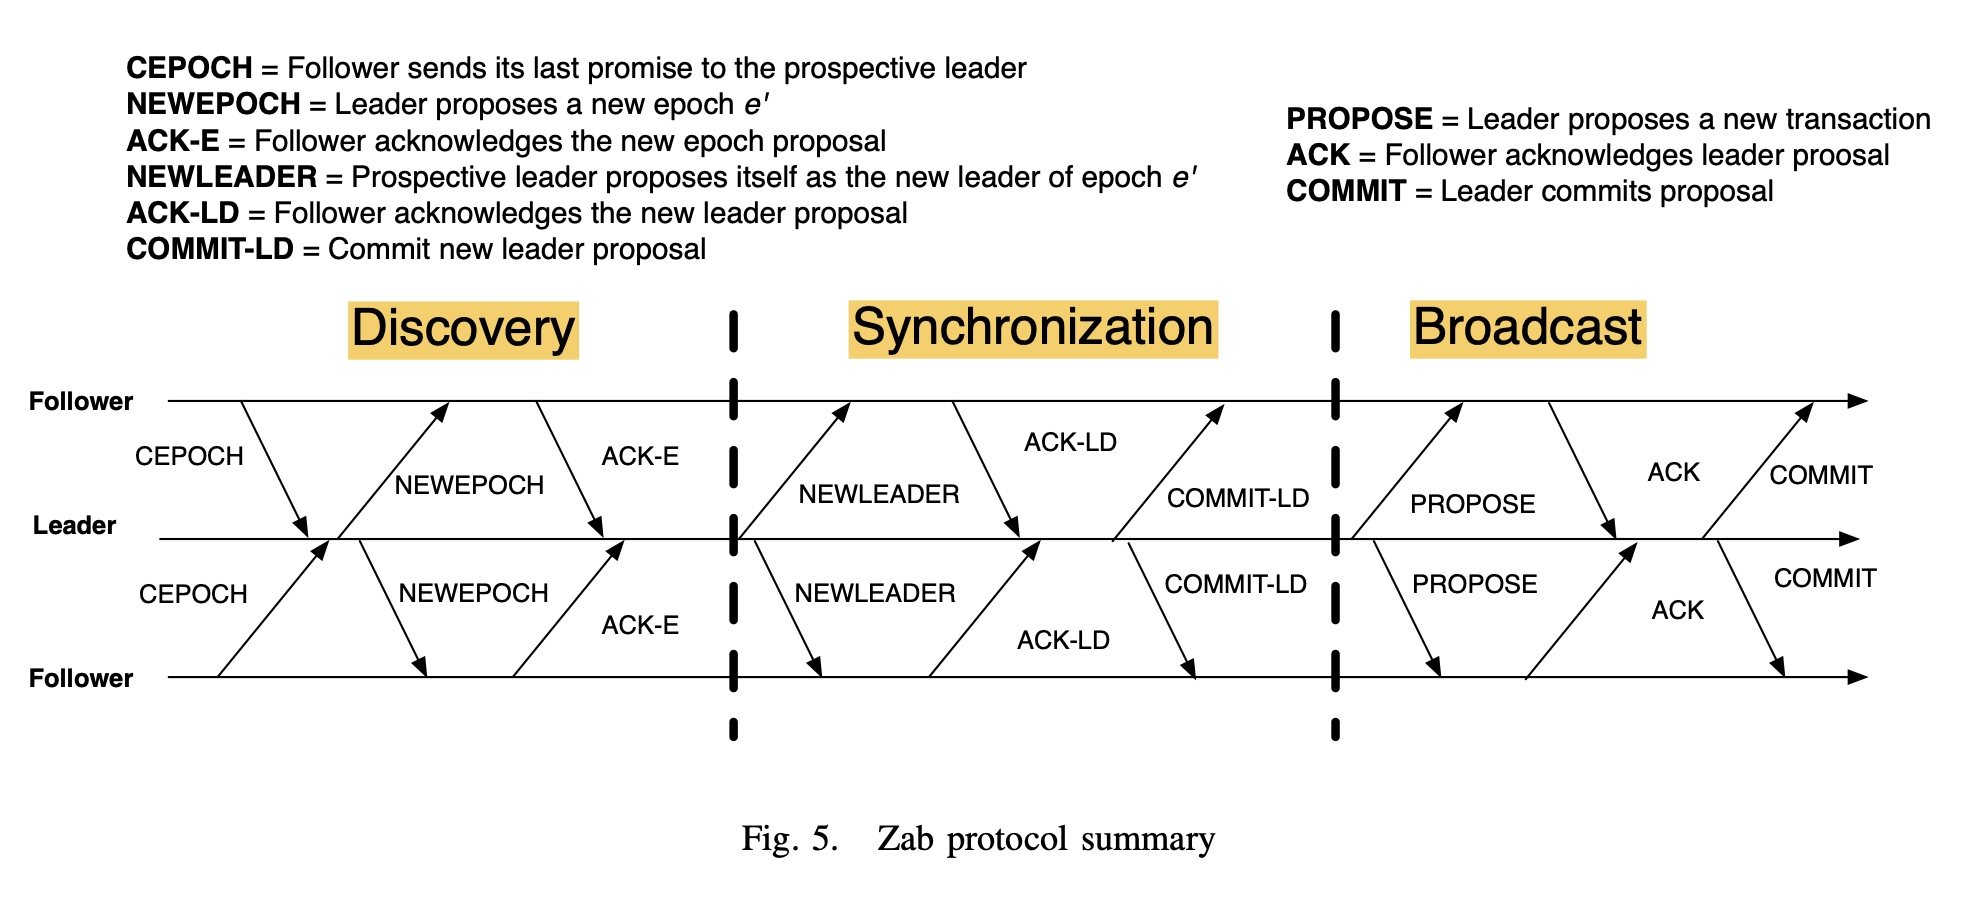
\includegraphics[scale=0.3]{diagrams/zab-protocol-overview.png}
\end{center}
Can see a TLA+ formal specificaton of the high level Zab protocol \href{https://github.com/apache/zookeeper/blob/248cc091d440659a819bdd44fe5b41a38321a929/zookeeper-specifications/protocol-spec/Zab.tla}{here}, which is a part of the official Apache Zookeeper repo.


\section{Byzantine Fault Tolerance}

The earliest explicit reference to \textit{Byzantine} faults appeared in \cite{1982lamportshostak}, though earlier work had touched on the same problem without referring to it by that moniker \cite{1980peasereaching,1978sift}. They show in \cite{1982lamportshostak} that when using ``oral'' messages (i.e. non-signed) messages, a Byzantine agreement solution requires $3f+1$ processes, even in a synchronous communication model. They give an algorithm that solves the problem assuming $n > 3f+1$, and also show that if we allow for ``written'' (e.g. digitally signed) messages, then in the synchronous model Byzantine agreement can be achieved with only $f+1$ processes.

\subsection{Model}
 
The work on Practical Byzantine Fault Tolerance (PBFT) \cite{1999castropbft} considers an asynchronous distributed system where nodes are connected by a network which can fail to deliver messages, delay them, or deliver them out of order. Furthermore, it allows for \textit{Byzantine} faults i.e., faulty nodes may behave arbitrarily, subject only to the above restrictions. This model does assume, however, cryptographic techniques that prevent spoofing and can detect corrupted messages. That is, Byzantine processes may send any arbitrary message, but we assume the identity of the sender of a message can be determined by the receiver \cite{2011lamport}. This can be achieved this with public-key signatures \cite{1978rivestcrypto}, message authentication codes (MACs), etc.

\subsection{Intuitions and Algorithm}

If we assume a starting point of a classic 2-phase Paxos consensus approach, the following are some of the essential issues that arise and must be dealt with when we add in Byzantine faults:
\begin{enumerate}
    \item \textbf{Leader equivocation}: if a leader is faulty (Byzantine), then it can trivially send two conflicting messages in the same view (i.e. with the same proposal number). This means that, for example, it could send out and accept messages with its own proposal number but with a different value to each replica. Then, we would end up with a quorum of replicas having accepted that proposal, but they all have different values, so which one is the true value to agree upon?
    \item \textbf{Wrong value adoption}: A leader (faulty or not) that accepts a wrong value  (i.e. not highest among previously) chosen can lead to safety violation as considered in the standard 2-phase Paxos model.
\end{enumerate}

Need to have a way for honest acceptor to only accept values if they have actually have proof that 


% A key idea of the algorithm is about how we deal with the issue of potentially Byzantine leaders. That is, we need to protect against leaders sending conflicting messages to different followers such that would violate the constraints needed to ensure safety in, for example, classic asynchronous consensus Paxos in the standard omission (non Byzantine) fault model.

\begin{itemize}
    \item If a leader/proposer is Byzantine, we can imagine it as not being a ``useful'' participant of the protocol, in that it may only be trying to be malicious. And, we can't control its behavior anyways, so we really need to worry about how acceptors can protect themselves against malicious leaders. 
    \item Normally, without Byzantine faults, acceptors can assume any incoming messages from proposers are legit, and they can respond with promises or acceptances accordingly.
    \item With Byzantine faults, though, the info they would hear from a proposer can't be trusted. So, can we force acceptors to somehow be more stringent in their acceptance of messages from proposers? In order to ensure they only actually accept messages from honest proposers?
    \item In essence, have proposers record the info they received from a large enough set of honest acceptors, in order to prove to an acceptor that this info was collected. Basically, let acceptors require that proposers prove to them that they collected info about prior acceptances from enough honest acceptors. Since we assume no forging possible we can have acceptors sign info accordingly in a way that proves they actually had a certain piece of info.
    \item \textbf{Point}: Acceptors will only accept if they have proof in the accept message that $X$ number of honest acceptors stored a particular proposal. 
    \item So, proposers first try to do their proposals by asking around acceptors, from which they receive promises. Then, the proposer sends out another round of ``real'' proposer
\end{itemize}



% If a leader is faulty and just went ahead and followed the standard 2-phase protocol used in Paxos (\textit{Prepare} + \textit{Accept}), then in the \textit{Prepare} phase it could tell different replicas arbitrarily different things i.e. tell them to accept one value and then change this value 

% \textbf{Note:} focus on reasoning about the protocol from ground up by looking at two special cases:
% \begin{itemize}
%     \item Faulty acceptors (can't trust 1b or 2b messages of classic Paxos since acceptors can lie)
%     \item Faulty proposers/leaders (can't trust 1a or 2a messages of classic Paxos since proposers can lie)
% \end{itemize}
% Need to have ways to protect against both scenarios. Generally, for the faulty acceptor case, we need to increase our quorum sizes in a way that ensures a propsoer can gather enough responses to be sure a sufficient number of honest responses were received. For faulty proposers, acceptors will need to implement some additional safety check to guard against proposers sending dishonest messages about values to be proposers/accepted.


% Why exactly is it bad if a leader is Byzantine i.e. even in classic Paxos?

The essence of the algorithm is as follows:
\begin{enumerate}
    \item Primary sends a $PrePrepare(value, p)$ message for view/proposal number $p$.
    \item Replica responds to the first $PrePrepare$ message it receives from a primary.
    \item Primary gathers $PrePrepare$ responses from $n-f$ replicas, and then sends $Prepare(v, proof)$ (note this message may be linear in size since it contains signed codes fro   m up to $n$ nodes.)
    \item If a replica sees $Prepare(value, p, proof)$ and $proof$ contains $n-f$ valid signatures for $PrePrepare(value, p)$, then it goes ahead and accepts.
    \item Primary then gathers $n-f$ $Prepare$ responses from replicas.
\end{enumerate}
Note that since we assume a public key infrastructure (PKI) set up between nodes of the system, any node can securely verify that a message was signed by some another node.

\subsection{Notes}
\begin{itemize}
    \item Given $n=3f+1$ nodes, for any 2 quorums with $n-f = 2f+1$ nodes, we are guaranteed they intersect in at least $f+1$ nodes (just draw a picture). Note that if you talk to at least $f+1$ nodes then you are sure you are in contact with at least one non-faulty (non-Byzantine) node.
\end{itemize}

\section{Blockchain and Cryptocurrency}

Decentralized currency have beomce a popular peer to peer consensus systems that operate under significantly different assumptions and fault models than previous systems.

\subsection{Bitcoin}

Bitcoin \cite{nakamoto2009bitcoin} is the first widely used decentralized cryptocurrency. Nodes participate in a peer-to-peer network that implements a distributed ledger which records all transactions between parties, which can be uniquely identified using cryptogaphic keys (e.g. RSA private keys). The ledger can be viewed as a type of database, consisting of a series of blocks that record transactions on the database. The current state of the database can be considered as the state of the ledger after applying all transactions in the ledger.

Generally, we can view our current (or most any) money system as, more or less, a big old database. As Buterin states in \cite{Buterin2013}:

\begin{quote}
    \dots all a currency, or token systen, fundamentally is is a database with one operation: subtract X units from A and give X units to B, with the proviso that: 
    \begin{enumerate}[(1)]
        \item A had at least X units before the transaction.
        \item The transaction is approved by A. 
    \end{enumerate}
\end{quote}

Every user/client of the database can have an account in this database, which records the current amount of money in their account (i.e. ``wallet''). Transactions are then executed by atomically transferring money from one account to another, by deducting some amount $X$ from user $A$'s account and adding $X$ to user $B$'s account, with the restriction that $A$ cannot send $X$ dollars to some other account if it does not have at least $X$ dollars. And, the transaction that completes between two accounts must occur atomically (consistently), before any other transactions take place. That is, we can think about all transactions as being serialized into a big list of transactions, which make up the \textit{ledger} or \textit{history} of the database. More generally, we can also consider this ledger itself as the current state of the database, since this state can always be computed by simply applying all transactions from the beginning of the ledger. We also might assume that there may be some special entries in this ledger that put new money into circulation by giving it to some account without requiring it to be transferred from an existing account.

If you try to build a money system on this decentralized ledger/database model, you have the obvious initial problem of how we update the database consistently and safely without the use of some central trusted authority. We can imagine that everyone has a copy of the full ledger, and can choose to make arbitrary updates to it locally e.g. even ones that break the \textit{no double spending} consistency property i.e., people could arbitrarily choose to spend money they don't have, breaking property 1 above. Additionally, we can assume that each party in the network can be uniquely identified by some cryptographic signing scheme e.g., each by their unique, private RSA key. They can mark a transaction between themselves, party $A$ and another user, party $B$, by referring to the public key of $B$ and signing the transaction with $A$'s private key. Based on this, other parties can then verify that $A$ was indeed the one who sent some money to $B$.

If everyone is updating their forks of the ledger independently, though, each with some potentially unsafe transactions, how do we enforce safety in a distributed fashion? Well, we must assume that there are at least some amount of honest nodes in the network that want to do good i.e., they are actually honest in wanting to only make sure that valid chains are kept in the system. Under this assumption, we can then use some mechanism that allows the honest agents to ``outvote'' the bad players when deciding on the correctness of the ledger. This can be implemented with the \textit{proof of work} concept. 

Basically, we imagine appending a special \textit{nonce} to each transaction, such that the original transaction concatenated with this nonce makes up the full transaction that goes into the chain. In order for a transaction be valid, though, we require some property of the hashed block be true that is computationally hard to invert. For example, by requiring that the SHA-256 hash of the original block plus the nonce starts with some number of zero bits. If this property holds true, then the transaction/block is considered valid, and this means fiddling with the data of the transaction would be computationally hard, since you would have to re-solve for a valid nonce. So, this implicitly ensures that votes are given to those with CPU power, and so if enough CPUs are ``honest'', then we have a good guarantee that honest nodes will win out in selecting the true ledger. 

\begin{center}
    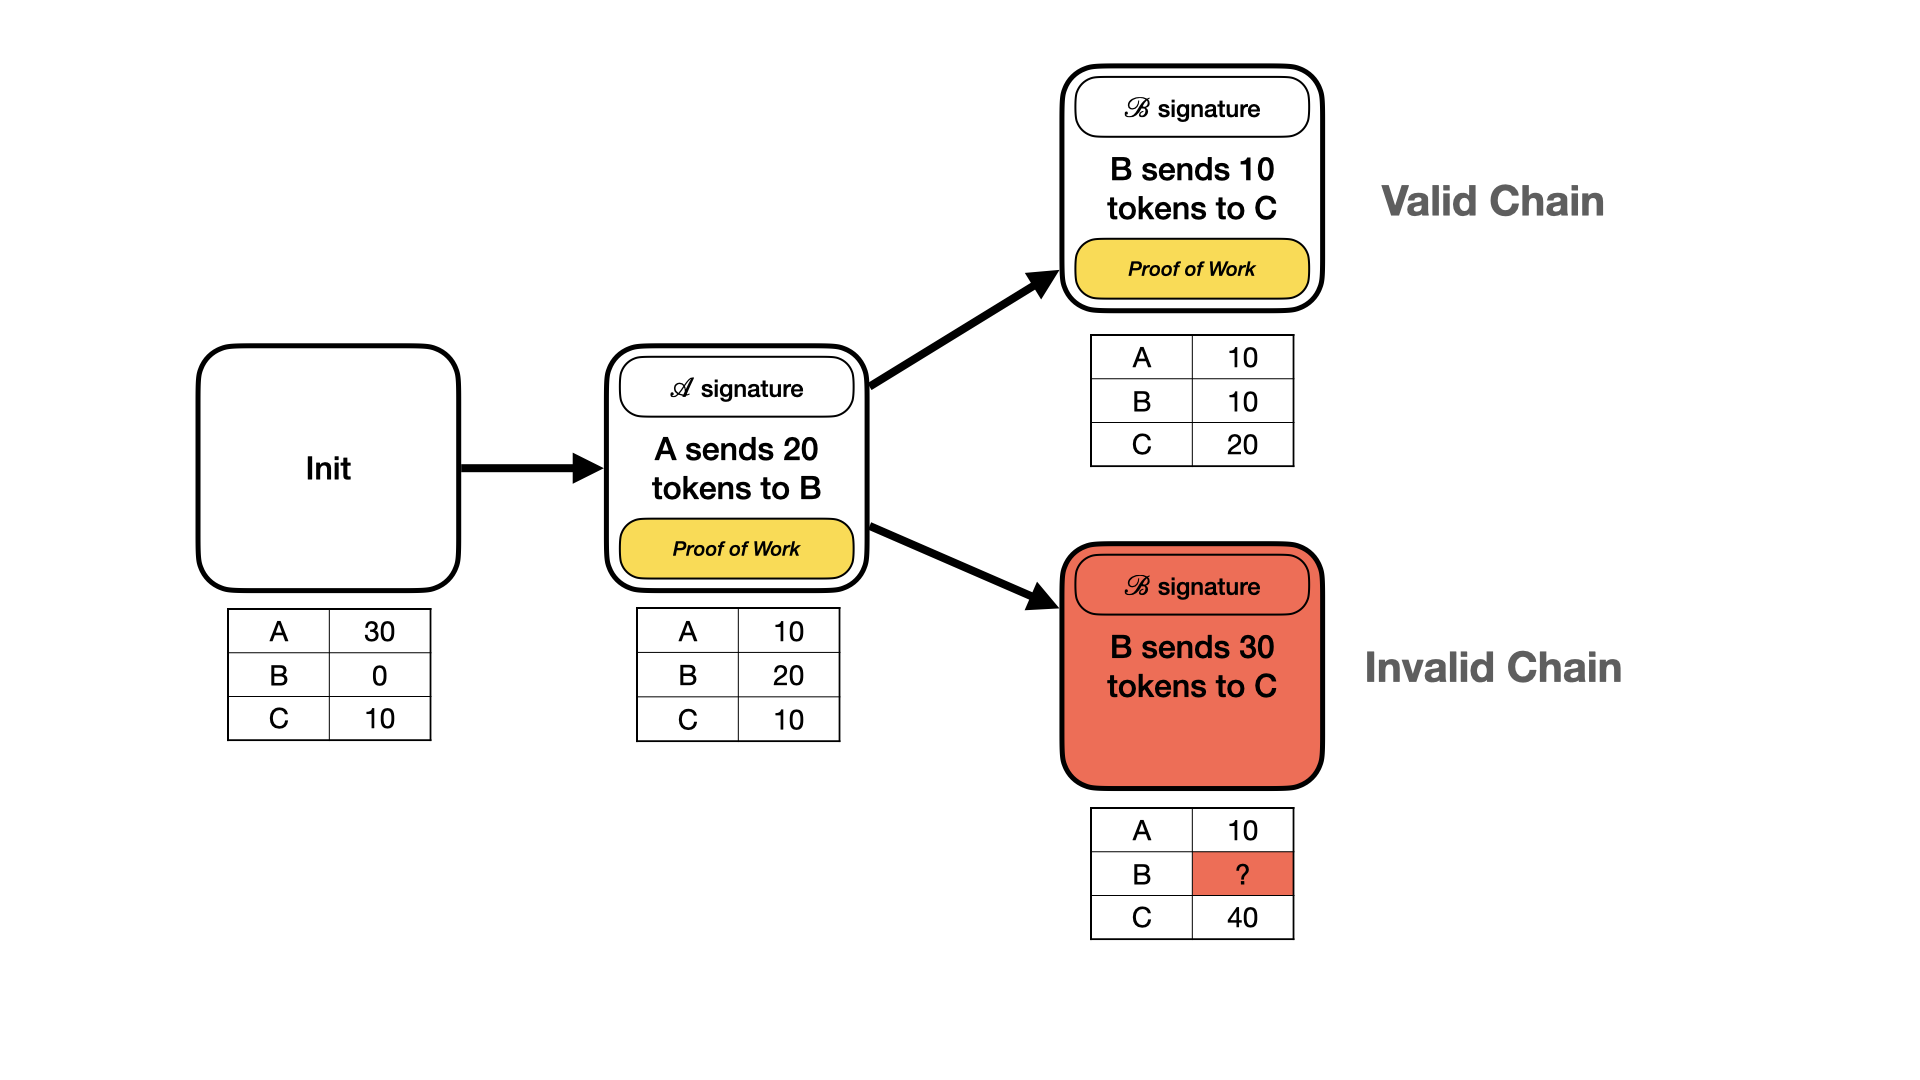
\includegraphics[scale=0.19]{diagrams/blockchain_diagrams/blockchain_diagrams.001.png}
\end{center}

In order to make a block ``valid'', you have to sign it with a special hash that is based on the block's content, and is computationally hard to come up with. This is the \textit{proof of work}. So, if you've sent out a valid block with a valid proof of work, it means you must have spent some amount of computational work on creating this block. This serves as the kind of ``voting'' power, allowing the larger pool of computational resources in the network to outvote any minority of bad actors, since, on average, this larger pool will win out in creating valid blocks and extending their chain.


\subsection{Ethereum}

Ethereum, originally published in a whitepaper \cite{Buterin2013} in 2014 by Vitalik Buterin, is a newer alternative to Bitcoin that is based on similar ideas and goals. Most notably, it introduces an explicit way to implement \textit{smart contracts} within the Ethereum blockchain, which allows for more elaborate financial contracts and transactions to be carried outbetween parties in the system. In a sense this is a kind of generalization of the basic banking \textit{state transition model} of Bitcoin, that only allowed users to essentially send value between each other without more complex contractual logic determining rules on how coins can flow between parties.

In Ethereum, the state is made up of objects called ``accounts'', which are each identifier by a 20-byte address and transactions are direct transfers of value and information between accounts. An Ethereum account contains four fields: (1) \textit{nonce}, a counter to ensure transactions are processed once, (2) \textit{ether balance}, the current balance of the account, (3) \textit{contract code}, if present, and (4) \textit{storage}, which is empty by default. There are then two different types of accounts:
\begin{enumerate}
    \item \textbf{Externally owned accounts}, which are controlled by private keys.
    \item \textbf{Contract accounts}, which are controlled by their contract code.
\end{enumerate}
Externally owned accounts have no code, and you can send messages from such an account by creating and signing a transaction. In a contract account, every time the contract account receives a message its code activates, allowing it to read and write to internal storage and send other messages or create contracts.

\subsubsection*{Messages and Transactions}

\textit{Messages} in Ethereum are similar to \textit{transactions} in Bitcoin, but differ in that an Ethereum message can be created either by an external entity or a contract, whereas a Bitcoin transaction can only be created externally. There is also an explicit option for Ethereum messages to contain data. Finally, the recipient of an Ethereum message, if it is a contract account, has the option to return a response, which means that Ethereum messages also encompass the concept of functions.

\textit{Transactions} in Ethereum contain the recipient of the message, a signature identifying the sender, the amount of ether and the data to send, as well as two values called \textit{STARTGAS} and \textit{GASPRICE}. To prevent exponential blowup and infinite loops in execution of contract code, each transaction is required to set a limit to how many computational steps of code execution it can spawn, including both the initial message and any additional messages that get spawned during execution. \textit{STARTGAS} is the limit on computational steps, and \textit{GASPRICE} is the fee to pay to the miner per computational step. 

% \subsubsection*{Smart Contracts}

% TODO.


\subsection{Blockchain Oracles}

Although smart contracts allow for secure, decentralized policies to be implemented within a blockchain network (e.g. in Ethereum) it is often the case that these contracts may want to use data sources that come from the outside wordl (e.g. stock stickers, weather, etc.). Mechanisms are needed for pulling in this data in a secure fashion, so that the security of the underlying contract is not compromised in cases where the external data source may also be compromised. A \textit{blockchain oracle} \cite{2016towncrier,breidenbach2021chainlink} is a third party service that connects a smart contract with the outside world, in an effort to address this issue.



\bibliographystyle{alpha}
\bibliography{../../references.bib}

\end{document}